\chapter{Desenvolvimento Teórico}

\section{Astrofografia}

%a \cite{livro:astropratica}

\subsection{Comprimento Focal}

\subsection{Exposição}
\subsubsection{Velocidade}
\subsubsection{Abertura}
\subsubsection{ISO}

\subsection{Formatos de Arquivos}

\subsection{Empilhamento de Fotos}

Softwares de empilhamento e soluções para pós processamento

\section{Plataformas Equatoriais}

\subsection{Métodos de Alinhamento Polar}

\subsubsection{Ajuste de Azimute}

\paragraph{Localização da Estrela Polar}
Uso de lunetas para alinhamento

\paragraph{Alinhamento com o Polo Norte}
Declinação Magnética

\subsubsection{Ajuste de Elevação}

%\subsubsection{Método \textit{Drift}}

\subsection{Soluções Comerciais Existentes}

Existem inúmeras soluções comerciais para o problema proposto, porém todos eles usam a luneta como método de alinhamento polar e isso só é praticável no hemisfério norte devido ao forte brilho da estrela polar diferentemente do situação no hemisfério sul. Existem produtos para todo o tamanho de orçamento. A tabela \ref{tabela_benchmark} ilustra a concorrência dos principais equipamentos, comparando as principais funcionalidades. 

\begin{table}[htb]
	\caption{Comparativo das Soluções de Mercado}
	\begin{tabular}{l|cccc}
		& Nyx Tracker & iOptron & Vixen Optics & SkyWatcher \\ \hline
		Preço (US\$) & 115 & 299 & 399 & 299 \\\hline
		Carga Máxima (kg) & 2.25 & 3 & 2 & 3 \\\hline
		Erro periódico (arcsec) & 115 & 100 & 50 & 50 \\\hline
		Volume $ (cm^2) $ & 155 & 490 & 323 & 220 \\\hline
		Peso (kg) & 0,4 & 1,15 & 0,79 & 0,72 \\\hline
		Alinhamento & \textit{Laser} & \textit{Polar Scope} & \textit{Polar Scope} & \textit{Polar Scope} \\
	\end{tabular}
	\label{tabela_benchmark}
	\fonte{\cite{site:nyxtech}}
\end{table}

Contudo, na realidade brasileira, o preço mostrado passaria ainda por impostos, tornando a compra mais inviável. O Nyx Tracker (Figura \ref{fig:nyxtracker}) é o sistema mais barato, com alinhamento impraticável no hemisfério sul, e também o mais simples em materiais.

\begin{figure}[h]
	\centering
	\caption{Nyx Tracker}
	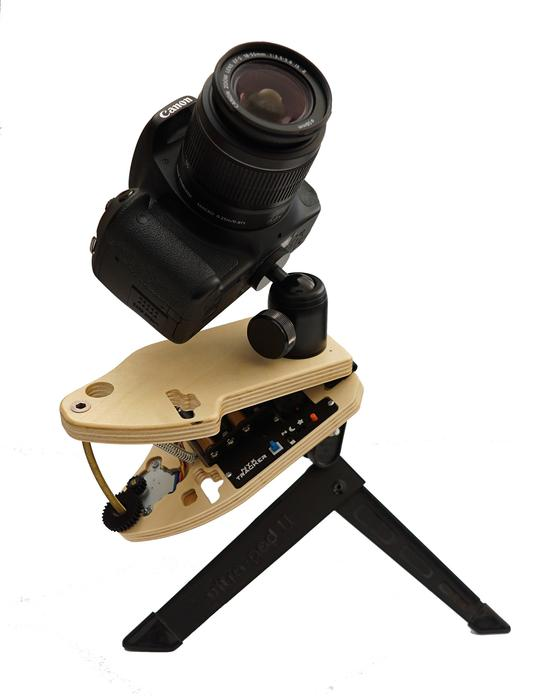
\includegraphics[width=0.3\linewidth]{figuras/nyxtracker}
	\label{fig:nyxtracker}
	\fonte{\cite{site:nyxtech}}
\end{figure}


\section{Objetivos}

Pelo \textit{benchmark} exposto, fixou-se como objetivos do sistema um produto robusto, visualmente elegante, e que consiga se aproximar das propriedades do modelo comercial mais barato, com erro periódico igual ou inferior a 115 arcsec, peso e volume adequados para o tripé usado, mantendo-se estável, sendo o menor possível e com o preço inferior a 115 dólares. Com o diferencial de um aplicativo que permita uma fácil interação do usuário com o sistema, descomplicando o processo.

\section{Protocolos de Comunicação}

\subsection{Serial}
\subsubsection{UART}
Velocidade, Falhas de comunicação, Guidelines de Design de PCB

\subsubsection{I2C}

Endereçamento, Velocidade, Guidelines de Design de PCB

\subsection{Bluetooth}

\section{Sensores e Atuadores}

\subsection{Acelerômetro}
\subsection{Giroscópio}
\subsection{Magnetômetro}

\subsection{GPS}

\subsection{Motor de Passo}

Driver, formas de Acionamento...

\section{Microcontroladores}

\subsection{Arduino Nano}

Justificativa, diagrama do Arduíno

\section{Interface Gráfica}

\subsection{Princípios e Diretrizes}

Os princípios e as diretrizes comumente utilizados em IHC giram em torno dos seguintes tópicos: correspondência com as expectativas dos usuários; simplicidade nas estruturas das tarefas; equilíbrio entre controle e liberdade do usuário; consistência e padronização; promoção da eficiência do usuário; antecipação das necessidades do usuário; visibilidade e reconhecimento; conteúdo relevante e expressão adequada; e projeto para erros.  \cite{BarbosaEtAl2021InteracaoHumanoComputadorExperiencia}
Esse conjunto de princípios são conhecidos como heurística de Nielsen, pois são aplicáveis em qualquer sistema, independente de casos específicos.

\subsubsection{Visibilidade dos status do sistema}

O sistema deve sempre manter o usuário atualizado sobre as condições de operação com uma taxa de atualização condizente para a informação. Ao informar o status da bateria, por exemplo, o usuário do smartphone consegue predizer quanto tempo de uso ainda terá e irá conseguir manejar sua interação com base nessa previsibilidade. \cite{site:nielsen}

\subsubsection{Comunicar-se com o mundo real}
O Design tem que se comunicar com o usuário na língua do usuário. Se um brasileiro não sabe inglês, ele ficará perdido nos Estados Unidos, pela mesma lógica, se a máquina não consegue se comunicar com o usuário, então ele ficará perdido.

Da mesma forma, o desenvolvedor não pode assumir que o usuário entenderá o aplicativo somente pelo fato do desenvolvedor ter feito algo que ele próprio entenda; é sempre preciso conferir a linguagem do sistema com um conjunto grande de pessoas para evitar mal entendidos, que se já ocorrem em língua nativa, na língua do sistema só tende a piorar.

Quando o usuário não entende a língua do sistema, ele se sente afastado e irá deixar de usar a plataforma. É interessante que a plataforma tenha designs semelhantes com objetos do mundo real, dessa forma, o usuário se sente "contemplado" e consegue facilmente fazer a conexão entre o mundo real e a plataforma. \cite{site:nielsenRealWorld}

\subsubsection{Liberdade de Controle do Usuário}

Por vezes, a pessoa que está realizando um processo em um sistema pode cometer um engano. Esse evento pode levar a situações de erro que não devem comprometer a experiência. Por isso, os usuários precisam de uma “saída de emergência” claramente marcada para sair do estado indesejado. Isso reduz a sua ansiedade e o medo de errar, pois ele sabe que os erros podem ser desfeitos. \cite{BarbosaEtAl2021InteracaoHumanoComputadorExperiencia}

\subsubsection{Consistências e Padrões}

É importante que o sistema mantenha uma consistência entre suas telas, ou mesmo em grandes plataformas, que os múltiplos programas tenham a mesma 'cara' com funções localizadas no mesmo lugar, com nomes similares e com um disign similar. Exeplo disso é as telas dos aplicativos do google docs; todos possuem o mesmo extilo de menu. MS Office também oferece isso.

A consistência também se extende aos ícones. O vetor que representa um botão, por exemplo, é importante que ele seja consistente em extilo com os demais. Eles podem ser mais preenchidos, mais \textit{clean}, mais neturos, mais suaves. O que importa mais nesse caso é que sejam todos padronizados. \cite{site:nielsenIcon}


\subsubsection{Prevenção de erros}

Uma forma de prevenção é oferecer sugestões numa caixa de pesquisa por exemplo. Em situações de rotina, como disparar um lembrete, a tela de criação pode oferecer uma sugestão defaut de template que faça sentido de fato para o usuário. Para evitar corrupção de dados pelo usuário na hora de um cadastro, é possível ofercer ao usuário que ele preencha números de uma forma truncada, e fazendo um pós processamento para ler o número corretamente.

\subsubsection{Relembrar o usuário é mais fácil do que o usuário relembrar}

Quando o usuário precisa repensar sobre algo incomoum na memória, ele precisa de muito tempo para pensar sobre esse algo. Então, quando a plataforma exige uma lembrança do usuário para entender algo, acaba que isso limita a experiência e incorre em perda de tempo, ou confusão.

Por isso, é mais interessante realizar a exigência com uma possível sugestão de resposta correta. A recognição de algo é muito mais prática para a mente humana pois ao mostrar para o cérebro algo relacionado com o que precisa lembrar-se, isso dispara a memória de forma mais forte. Dar uma pista para o cérebro é mais eficiente do que simplesmente perguntar sem oferecer nada para a memória. \cite{site:nielsenRecall}

\subsubsection{Torne o sistema flexível e eficiente}

Atalhos, personalização e customização. Com esses 3 fatores é possível melhorar a usabilidade para aqueles que não são mais novatos no software e isso ajuda a manter esses usuários ativos. Um fotógrafo experiente, que está acostumado com os atalhos de teclado nos aplicativos da Adobe, teria muita "dor de cabeça" se o teclado viesse a falhar, pois a mente já assimilou os atalhos mais usados e eles fazem diferença na velocidade com que o profissional atua com o software.
\cite{site:nielsenFlexibility}

\subsubsection{Tenha um Design minimalista}

Um design minimalista ajuda a ter somente o que é necessário focar na tela, isso ajuda o usuário a não se sentir perdido. Isso significa usar elementos simples num arranjo onde desenho e a interface combine de forma agradável sem chamar a atenção de forma desnecessária. \cite{site:nielsen}

\subsubsection{Ajude o usuário a entender e se recuperar de erros}

O usuário precisa entender quando o sistema não está funcionando bem e como fazê-lo voltar ao normal. As mensagens de erro devem ser expressas em de uma forma simples, indicando o possível problema e a solução. 
Cores vermelhas e pretas ajudam a demonstrar o sinal de erro para o usuário. \cite{site:nielsenError}

\subsubsection{Tire dúvidas e documente o sistema}

Existem duas formas de ajudar o usuário e tirar suas dúvidas. A primeira é de forma proativa, onde a aplicação guia o usuário para se familiarizar com a interface. Outra forma é por meio de uma seção com perguntas e respotas, essa seção ajuda os usuários a se tornarem mais independetes com a aplicação, resolvendo seus próprios problemas e filtrando os casos que precisam de suporte para a equipe técnica da plataforma. \cite{site:nielsenHelpandDoc}

\subsection{Android}
\subsubsection{Ambiente de Desenvolvimento}

O \textit{Android Studio} é o ambiente de desenvolvimento integrado oficial para a criação de apps \textit{Android} e é baseado no \textit{IntelliJ IDEA}. Ele oferece uma série de Recursos que possibilitam a confecção de um aplicativo: Sistema de compilação flexível baseado em \textit{Gradle}; Um emulador rápido com suporte a vários recursos; um ambiente unificado que possibilita o desenvolvimento para qualquer dispositivos Android, incluindo relógios e televisões; Integração com GitHub para backup e documentação do código; entre outras funções que possibilitam análizar o desempenho de um aplicativo em tempo real, bem como fazer updates. \cite{site:androidstudio}

\subsubsection{Linguagens de Programação}

Existem soluções de desenvolvimento Android mais \textit{user-friendly} como \textit{APP Inventor} ou \textit{Kodular}, porém, essas interfaces não garantem ao desenvolvedor um pleno controle do aplicativo, e muitas vezes acaba limitando a interface. Por isso, usar linguagens de programação nativas é uma abordagem mais interessante para aplicativos mais completos. É possível criar aplicativos com diversas linguagens, mas somente duas são nativas e permitem realizar aplicações que podem abusar de todo o poder de processamento de um \textit{smartphone}: Java e Kotlin.

Em 2017, Kotlin foi definido pela Google como sendo a principal linguagem de desenvolvimento Android. A linguagem ainda é muito mais nova que Java, sendo desenvolvida em pela JetBrains. As grandes motivação de se usar Kotlin para o desenvolvimento reside nos fatos de ser uma linguagem segura para prevenção de objetos nulos, operando em paralelo com qualquer código em Java e dando opções de co-rotinas. Além disso, ao comparar dois códigos com a mesma função, um escrito em Java, outro em Kotlin; o segundo pode ser até 40\% mais compacto, o que implica em uma linguagem mais concisa e compreensível entre desenvolvedores. As desvantagens de se usar Kotlin, para este trabalho, é somente a falta de uma comunidade grande, comparando com Java; o que limita o suporte para eventuais problemáticas de desenvolvimento. \cite{site:kotlinxjava}

Dentro do ambiente de Desenvolvimento usa-se também linguagem de arquivos XML para a criação de interfaces gráficas (\textit{layouts}) bem como a escrita dos vetores, animações, e arquivos de configuração do aplicativo e temas de \textit{layout}. Para armazenamento de dados dentro do aplicativo normalmente usa-se uma \textit{database} que é operada com códigos de consulta \textit{SQL}.

\subsubsection{\textit{Material Design}}
Existem uma série de diretrizes de Design fornecidas pela Google para guiar o desenvolvimento de aplicativos android. Essas informações são fornecidas principalmente pela biblioteca Material Design, que fornece pacotes facilmente implementáveis de layouts para aplicações responsivas e padronizadas.

A Biblioteca colabora com o desenvolvedor fornecendo icones, tipografia, cores e componentes gráficos que trazem uma imersão para o usuário de forma simples e minimalista. Os design se inspiram no mundo real, facilitando a comunicação com o usuário. \cite{site:materialdesign}



